

\tikzset{every picture/.style={line width=0.75pt}} %set default line width to 0.75pt        

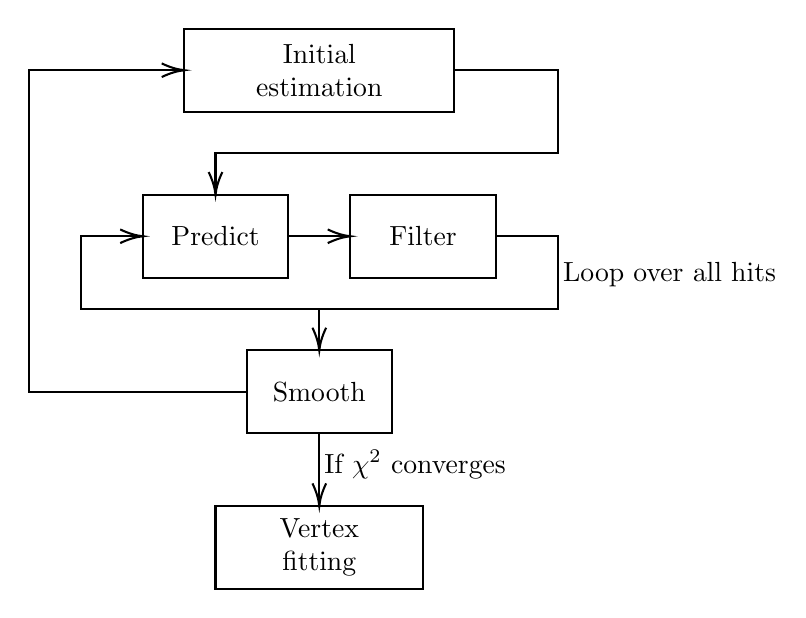
\begin{tikzpicture}[x=0.75pt,y=0.75pt,yscale=-1,xscale=1]
%uncomment if require: \path (0,359); %set diagram left start at 0, and has height of 359

%Shape: Rectangle [id:dp9978340606054834] 
\draw   (205,20) -- (335,20) -- (335,60) -- (205,60) -- cycle ;
%Shape: Rectangle [id:dp36333722789056344] 
\draw   (185,100) -- (255,100) -- (255,140) -- (185,140) -- cycle ;
%Shape: Rectangle [id:dp8065489263231345] 
\draw   (285,100) -- (355,100) -- (355,140) -- (285,140) -- cycle ;
%Shape: Rectangle [id:dp3416154088376071] 
\draw   (235,175) -- (305,175) -- (305,215) -- (235,215) -- cycle ;
%Shape: Rectangle [id:dp4411494772649741] 
\draw   (220,250) -- (320,250) -- (320,290) -- (220,290) -- cycle ;
%Straight Lines [id:da7344533518933397] 
\draw    (335,40) -- (385,40) -- (385,80) -- (220,80) -- (220,98) ;
\draw [shift={(220,100)}, rotate = 270] [color={rgb, 255:red, 0; green, 0; blue, 0 }  ][line width=0.75]    (10.93,-3.29) .. controls (6.95,-1.4) and (3.31,-0.3) .. (0,0) .. controls (3.31,0.3) and (6.95,1.4) .. (10.93,3.29)   ;
%Straight Lines [id:da06782376989613081] 
\draw    (255,120) -- (283,120) ;
\draw [shift={(285,120)}, rotate = 180] [color={rgb, 255:red, 0; green, 0; blue, 0 }  ][line width=0.75]    (10.93,-3.29) .. controls (6.95,-1.4) and (3.31,-0.3) .. (0,0) .. controls (3.31,0.3) and (6.95,1.4) .. (10.93,3.29)   ;
%Straight Lines [id:da03444837242423393] 
\draw    (355,120) -- (385,120) -- (385,155) -- (155,155) -- (155,120) -- (183,120) ;
\draw [shift={(185,120)}, rotate = 180] [color={rgb, 255:red, 0; green, 0; blue, 0 }  ][line width=0.75]    (10.93,-3.29) .. controls (6.95,-1.4) and (3.31,-0.3) .. (0,0) .. controls (3.31,0.3) and (6.95,1.4) .. (10.93,3.29)   ;
%Straight Lines [id:da9288077865829715] 
\draw    (270,155) -- (270,173) ;
\draw [shift={(270,175)}, rotate = 270] [color={rgb, 255:red, 0; green, 0; blue, 0 }  ][line width=0.75]    (10.93,-3.29) .. controls (6.95,-1.4) and (3.31,-0.3) .. (0,0) .. controls (3.31,0.3) and (6.95,1.4) .. (10.93,3.29)   ;
%Straight Lines [id:da9916095919187531] 
\draw    (235,195) -- (130,195) -- (130,40) -- (203,40) ;
\draw [shift={(205,40)}, rotate = 180] [color={rgb, 255:red, 0; green, 0; blue, 0 }  ][line width=0.75]    (10.93,-3.29) .. controls (6.95,-1.4) and (3.31,-0.3) .. (0,0) .. controls (3.31,0.3) and (6.95,1.4) .. (10.93,3.29)   ;
%Straight Lines [id:da7888302009088826] 
\draw    (270,215) -- (270,248) ;
\draw [shift={(270,250)}, rotate = 270] [color={rgb, 255:red, 0; green, 0; blue, 0 }  ][line width=0.75]    (10.93,-3.29) .. controls (6.95,-1.4) and (3.31,-0.3) .. (0,0) .. controls (3.31,0.3) and (6.95,1.4) .. (10.93,3.29)   ;

% Text Node
\draw (270,40) node   [align=left] {\begin{minipage}[lt]{72.76pt}\setlength\topsep{0pt}
\begin{center}
Initial estimation
\end{center}

\end{minipage}};
% Text Node
\draw (220,120) node   [align=left] {\begin{minipage}[lt]{34pt}\setlength\topsep{0pt}
\begin{center}
Predict
\end{center}

\end{minipage}};
% Text Node
\draw (320,120) node   [align=left] {\begin{minipage}[lt]{24.48pt}\setlength\topsep{0pt}
\begin{center}
Filter
\end{center}

\end{minipage}};
% Text Node
\draw (270,195) node   [align=left] {\begin{minipage}[lt]{37.4pt}\setlength\topsep{0pt}
\begin{center}
Smooth
\end{center}

\end{minipage}};
% Text Node
\draw (270,270) node   [align=left] {\begin{minipage}[lt]{55.76pt}\setlength\topsep{0pt}
\begin{center}
Vertex fitting
\end{center}

\end{minipage}};
% Text Node
\draw (386,131) node [anchor=north west][inner sep=0.75pt]   [align=left] {Loop over all hits};
% Text Node
\draw (271,230) node [anchor=west] [inner sep=0.75pt]   [align=left] {If $\displaystyle \chi ^{2}$ converges};


\end{tikzpicture}

